\capitulo{3}{Conceptos teóricos}

A continuación, se explican algunos conceptos teóricos que ayudan a comprender mejor el trabajo realizado.

\section{Conceptos teóricos básicos}

\subsection{Aprendizaje automático}
El aprendizaje automático o \textit{machine learning} es un enfoque de la IA que permite a un sistema resolver diversas tareas aprendiendo patrones a partir de los datos de entrenamiento y automatizando el proceso de construcción de modelos analíticos ~\cite{janiesch2021machine}.

\begin{figure}[h]
    \centering
    
\includegraphics[width=0.40\textwidth]{img/Aprendizaje automatico.png}
    \caption{Inteligencia artifical, \textit{deep learning} y \textit{machine learning}\\  ~\cite{UniMa24}}
    \label{fig:aprendizaje_automatico}
\end{figure}
\FloatBarrier

\subsubsection{Aprendizaje profundo}
El aprendizaje profundo es un concepto de aprendizaje automático basado en redes neuronales artificiales ~\cite{janiesch2021machine} tal y como se puede apreciar en la figura \ref{fig:aprendizaje_automatico}.

En el aprendizaje profundo, la extracción de características se hace a partir de un conjunto de datos en bruto empleando múltiples capas ocultas mientras que, en el aprendizaje automático, esta extracción se realiza de forma manual, como paso previo al modelamiento\\ ~\cite{diego23}. 

Es decir, en el aprendizaje profundo las características se extraen automáticamente de los datos de entrada y se clasifican. Por otro lado, en el aprendizaje automático las características se extraen de forma manual para su clasificación o segmentación ~\cite{kundu2021pneumonia}.

El aprendizaje profundo emplea una mayor cantidad de datos y un mejor rendimiento que el aprendizaje automático\\ ~\cite{diego23}.


Entre los tipos de aprendizaje profundo se encuentran:
\begin{itemize}
    \item \textbf{Aprendizaje supervisado}: proporciona al algoritmo unos datos de entrada que, contienen las características de los datos que serán procesados y una etiqueta que los define, lo que permite, tanto entrenar un algoritmo como evaluarlo. Las CNN, las redes neuronales recurrentes o las arquitecturas tipo codificador-decodificador son ejemplos de modelos que emplean este tipo de aprendizaje\\ ~\cite{diego23}.
    \item \textbf{Aprendizaje no supervisado}: el conjunto de datos que proporciona al algoritmo está sin procesar y sin etiquetar\\ ~\cite{sindhu2020survey}. Por lo tanto, a la hora de clasificar el conjunto de datos de entrada en diversas clases, el algoritmo tendrá que identificar los patrones que caracterizan a los datos sin una referencia específica. Los algoritmos de clusterización son un ejemplo de aprendizaje no supervisado ~\cite{diego23}.
    \item \textbf{Aprendizaje por refuerzo}: aprende a realizar diversas acciones a partir de una realimentación de recompensas o penalizaciones\\ ~\cite{diego23}.
\end{itemize}

\textbf{Redes neuronales artificiales (RNA)}

Como ya se ha comentado previamente, las CNN emplean el aprendizaje profundo supervisado dentro del dominio de la IA. 

Una RNA es un paradigma de procesamiento de información para el reconocimiento de patrones y la predicción a partir de neuronas interconectadas inspiradas en el cerebro humano ~\cite{walczak2019artificial}.

El desarrollo de las RNA comenzó con la propuesta de McCulloch y Pitts (1943) de un modelo matemático de actividad neuronal en el cerebro ~\cite{walczak2019artificial}.

Los principales componentes de las redes neuronales artificiales, los cuales se pueden ver en la figura \ref{fig:w_b}, son:

\begin{figure}[h]
    \centering
    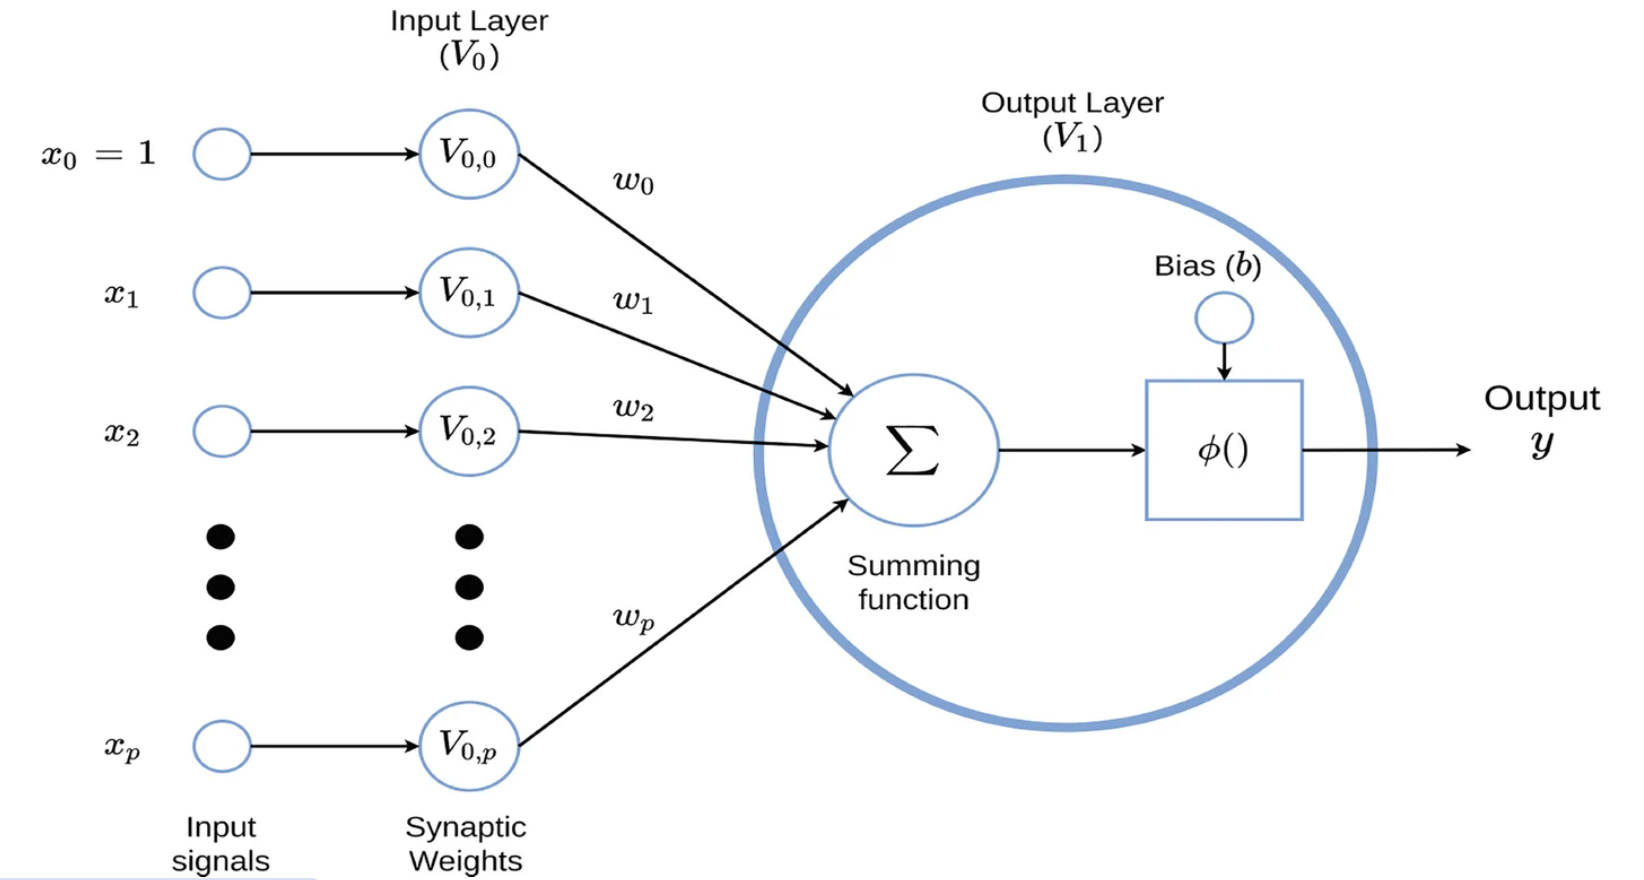
\includegraphics[width=0.99\textwidth]{img/w_b.PNG}
    \caption{Ilustración red neuronal artificial  ~\cite{montesinos2022fundamentals}}
    \label{fig:w_b}
\end{figure}
\FloatBarrier

\begin{itemize}
    \item \textbf{x1,...,xp}: es la información o señales de entrada que puede recibir la neurona tanto del sistema sensorial externo como de otras neuronas con las que tiene conexión ~\cite{montesinos2022fundamentals}.
    \item \textbf{Parámetros ``w'' (w1,...,wp)}: Es el vector de pesos sinápticos que mide la eficiencia con que la sinapsis afecta el potencial de la neurona ~\cite{montesinos2022fundamentals}. Se emplea y ajusta durante el proceso de entrenamiento para que la red neuronal pueda realizar predicciones de forma precisa ~\cite{diego23}. 
    \item \textbf{Parámetro ``b''}: Es el sesgo o umbral que se emplea para equilibrar el valor medio de las entradas con el valor medio de las salidas deseadas. Al igual que el parámetro ``w'', el parámetro ``b'' también se emplea y ajusta durante el proceso de entrenamiento para que la red neuronal pueda realizar predicciones de forma precisa~\cite{diego23}. 
\end{itemize}


\subsection{Época}
A la hora de entrenar un modelo, se realizan múltiples iteraciones sobre el conjunto de datos con un determinado tamaño de lote o \textit{batch size} (explicado a continuación), actualizando en cada iteración los parámetros ``w'' y ``b''. A estas iteraciones se las conoce como épocas\\ ~\cite{diego23}.

\subsection{\textit{Batch size}}
También denominado ``tamaño de lote'', se trata de un hiperparámetro que define el número de muestras de entrenamiento introducidas en la red para cada iteración ~\cite{link24}. Por ejemplo, si se elige un \textit{batch size}=100 y se tiene un tamaño de muestra de 2050, el algoritmo coge las muestras de 100 en 100 para entrenar la red. Es decir, toma las primeras 100 muestras y entrena la red, a continuación, coge las siguientes 100 y así sucesivamente hasta terminar con el número de muestras. En este caso, al no ser divisible el número de muestras entre 100, la solución más sencilla sería, en el último entrenamiento coger las 50 muestras restantes y entrenar la red ~\cite{stack24}.

El valor de \textit{batch size} elegido para entrenar la red tiene un impacto importante en la precisión, velocidad y estabilidad. Un \textit{batch size} mayor, indica que se procesan un mayor número de muestras en paralelo, lo que disminuye el tiempo de ejecución e implica una mayor eficiencia computacional, pero, también requiere una gran cantidad de memoria y, puede afectar a la generalización y convergencia del modelo pudiendo generar un sobreajuste, lo que puede ser un inconveniente en algunos sistemas. Por otro lado, un \textit{batch size} menor, permite actualizaciones más frecuentes de los pesos y una mejor generalización, además de un menor uso de memoria y puede evitar el sobreajuste, pero, requiere un mayor tiempo de entrenamiento, la eficiencia computacional es reducida y aumenta el ruido en las estimaciones de gradiente ~\cite{link24}. Por lo tanto, a la hora de elegir el mejor \textit{batch size}, se tiene que encontrar un equilibrio entre precisión y tiempo de entrenamiento.

Por todo esto, el \textit{batch size} óptimo varía según la red neuronal. Es importante probar diferentes valores de \textit{batch size} y comprobar cómo este afecta al rendimiento del modelo durante el entrenamiento. 

\subsection{\textit{Padding}}

\textit{Padding} es uno de los argumentos empleados tanto en la capa convolucional (Conv2D) como en la capa MaxPooling2D para realizar la convolución entre el filtro y la imagen de entrada a la hora de cear el modelo. La convolución consiste en aplicar un filtro (también denominado kernal) a una imagen para extraer características específicas ~\cite{diego23}.

Su objetivo principal es añadir pixeles alrededor de los bordes de la imagen de entrada. Los valores que se añaden son ceros (tal y como se puede apreciar en la figura \ref{fig:padding}) o los mismos valores del borde inicial de la imagen ~\cite{diego23}.

\begin{figure}[h]
    \centering
    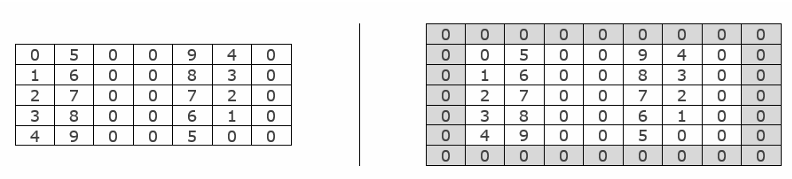
\includegraphics[width=0.99\textwidth]{img/padding.PNG}
    \caption{\textit{Padding} añadiendo ceros ~\cite{diego23}}
    \label{fig:padding}
\end{figure}
\FloatBarrier

Las opciones válidas para el argumento \textit{padding} son ``\textit{valid}'' y ``\textit{same}''. Donde ``\textit{valid}'' significa que no se aplica \textit{padding} y ``\textit{same}'' realiza el \textit{padding} de forma que, la dimensión de salida de la capa de convolución sea la misma que la de entrada ~\cite{diego23}.

\subsection{\textit{Stride}}

\textit{Stride} es otro argumento empleado tanto en la capa convolucional (Conv2D) como en la capa MaxPooling2D a la hora de crear el modelo. Se corresponde con el número de columnas y filas que se desplaza el kernal en cada operación ~\cite{diego23} tal y como se muestra en la figura \ref{fig:stride}.

\begin{figure}[h]
    \centering
    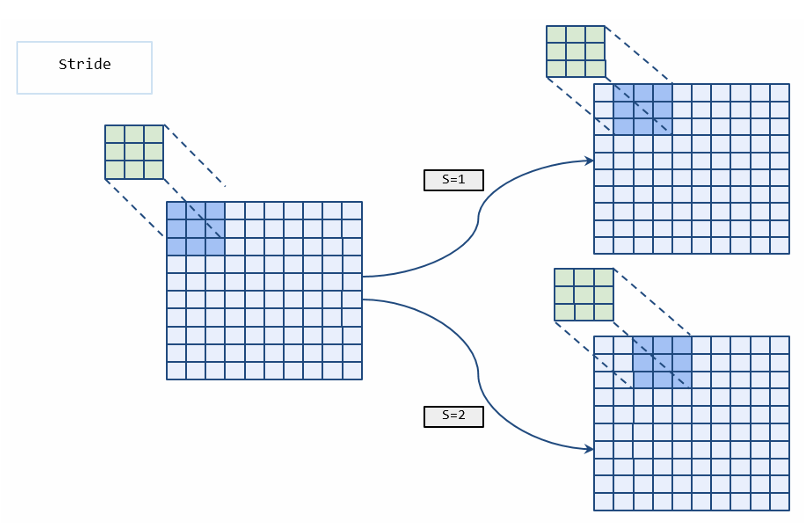
\includegraphics[width=0.99\textwidth]{img/stride.PNG}
    \caption{\textit{Stride} con valores 1 y 2 ~\cite{diego23}}
    \label{fig:stride}
\end{figure}
\FloatBarrier

Para definir \textit{stride} en keras, se debe indicar un valor entero o una tupla de dos enteros. En el caso de indicar un número entero, significa que el filtro se desplaza el mismo número para filas y columnas. Sin embargo, si se introduce una tupla, el número de filas y columnas es distinto ~\cite{diego23}.

\subsection{\textit{Overfitting}}
\textit{Overfitting} o sobreajuste, ocurre cuando el error de entrenamiento es mucho menor que el error de validación. Es decir, el clasificador tiene un error de entrenamiento muy bajo puesto que se ajusta demasiado a los datos de entrenamiento, pero, sin embargo, no es capaz de generalizar en el conjunto de validación ~\cite{diego23}.  Esto es un problema dado que, al entrenar redes neuronales, interesa que, no solo sea capaz de ajustarse correctamente a los modelos de entrenamiento, sino que también, a datos nuevos con los que se quiera trabajar. Por ello, a la hora de entrenar una red neuronal, además de los datos de entrenamiento, también se cuenta con un ``conjunto de prueba'' o ``\textit{train data}'' y uno de validación o ``\textit{validation data}''. 


\begin{figure}[h]
    \centering
    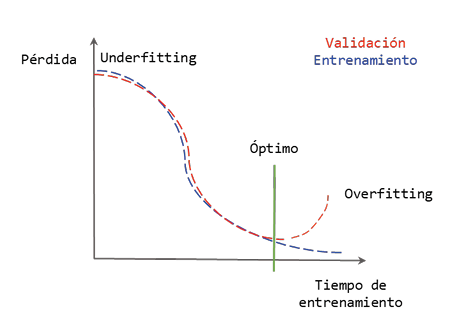
\includegraphics[width=0.70\textwidth]{img/sobreajuste.PNG}
    \caption{Ilustración del sub-ajuste (\textit{underfitting}) y sobreajuste (\textit{overfitting}) en modelos de aprendizaje automático\\ ~\cite{diego23}}
    \label{fig:sobreajuste}
\end{figure}
\FloatBarrier

Por el contrario, el \textit{underfitting} o sub-ajuste, ocurre cuando el modelo no se ajusta de forma correcta al conjunto de entrenamiento y, a su vez, tanto el error en el conjunto de entrenamiento como en el conjunto de validación es muy similar ~\cite{diego23}.

El sobreajuste está muy relacionado con el tamaño y la complejidad del modelo dado que, el modelo puede aprender el ``ruido'' o información irrelevante de los datos, lo que provoca que el modelo no pueda generalizar correctamente nuevos datos y, por tanto, no realice una buena predicción ~\cite{ibm24}.

Para reducir el sobreajuste se emplean tácticas como el aumento de los datos de entrenamiento (en número y diversidad), la reducción de la complejidad del modelo, añadir criterios de detección temprana como ``\textit{Early Stopping}'', modificar los atributos de entrada o agregar técnicas de regulación entre otras ~\cite{diego23}. 

\subsection{\textit{Early Stopping}}
Se trata de una técnica de reducción de \textit{overfitting} con la cual se agrega un criterio de detención temprana para detener el entrenamiento de forma anticipada ~\cite{diego23}.

\textit{Early Stopping} monitorea el rendimiento del conjunto de validación durante el entrenamiento y, detiene el proceso de entrenamiento cuando el rendimiento del conjunto de validación comienza a empeorar ~\cite{keras24}. Tal y como se puede apreciar en la imágen \ref{fig:sobreajuste} que aparece en la página \pageref{fig:sobreajuste} donde, la línea azul representa el conjunto de entrenamiento y la roja el conjunto de validación. La línea verde dónde pone ``óptimo'', corresponde con el punto donde \textit{Early Stopping} detendrá el entrenamiento ya que, aunque la línea del conjunto de entrenamiento continúa disminuyendo (es decir, el error o pérdida se acerca a 0), la línea del conjunto de validación comienza a ir en aumento, lo que significa que empeora.

Entre los principales argumentos incluidos a la hora de definir \textit{EarlyStopping}, se encuentra ``\textit{patience}'', el cual indica el número de épocas que tienen que pasar sin mejora para que, el entrenamiento se detenga ~\cite{keras24}. Este argumento se incluye para dejar algo de margen en el conjunto de validación en el caso de que empeore en un momento dado, pero, al cabo de un número pequeño de épocas o iteraciones vuelva a mejorar. 

\subsection{Radiografía de Rayos X}

La radiografía es una técnica de diagnóstico por imágenes que emplea rayos X para producir imágenes de las estructuras internas del cuerpo. A partir de estas imágenes, los profesionales pueden examinar y diagnosticar diversas afecciones como cáncer, roturas, problemas en los órganos internos, etc ~\cite{CliUniNa24}. Se emplea para analizar diversas parte del cuerpo pero en especial, el abdomen, tórax, huesos y dientes ~\cite{Macli24}.

Las imágenes se forman a partir del bloqueo de la radiación que producen los diferentes tejidos y estructuras del cuerpo según su densidad. Al colocar la parte del cuerpo donde se va a realizar la radiografía, entre la fuente de rayos X y la placa, se disparan los rayos X y, en la placa aparece los rayos X que han pasado según la zona. Por ejemplo, los materiales densos como huesos o metales, se observaran como zonas blancas debido a que bloquean mejor los rayos X mientras que, el aire se observara como una zona oscura ya que, no es capaz de bloquearlos ~\cite{CliUniNa24, Macli24}.

Cabe mencionar que, aunque la radiografía es de gran ayuda en algunos casos por ser un método rápido, no invasivo, de bajo coste y amplia disponibilidad, también presenta algunas limitaciones. En ocasiones, puede que en la imagen no se vea correctamente todo lo que se debería ver, como, por ejemplo, algunos tejidos blandos como tendones, músculos o ligamentos. Para estos casos se emplea la ecografía, RM o TC ~\cite{CliUniNa24}.

Los avances tecnológicos y científicos, han hecho posible la realización de radiografías con la mínima radiación posible, aumentando la seguridad del paciente a la hora de realizar este tipo de pruebas ~\cite{CliUniNa24}. 

Para más información acerca de las radiografías de rayos X consultar \textit{Anexo D}.


\subsubsection{Radiografía de tórax (CXT por sus siglas en inglés)}

La CXT es la base de las imágenes para el cribado pulmonar\\ ~\cite{gelaw15}. Con ella, se puede comprobar si existe algún problema en los pulmones, el corazón o la pared del pecho ya que, se observan los órganos y estructuras del interior del tórax\\ ~\cite{Macli24, NIH24}.

A la hora de realizar una CXT, la posición más común es la proyección postero anterior (PA), donde el paciente debe colocarse de pie en posición vertical frente a la placa de imagen. Los pies se colocan ligeramente separados para una mayor estabilidad del paciente. Las manos se colocan en las caderas y los codos hacia delante. El tórax debe estar alineado con la placa de la imagen ~\cite{gelaw15}. Esto se puede observar mejor en la figura \ref{fig:radiografia torax}. Para saber más acerca de otras vistas posibles en la CXT consultar \textit{Anexo D}.

\begin{figure}[h]
    \centering
    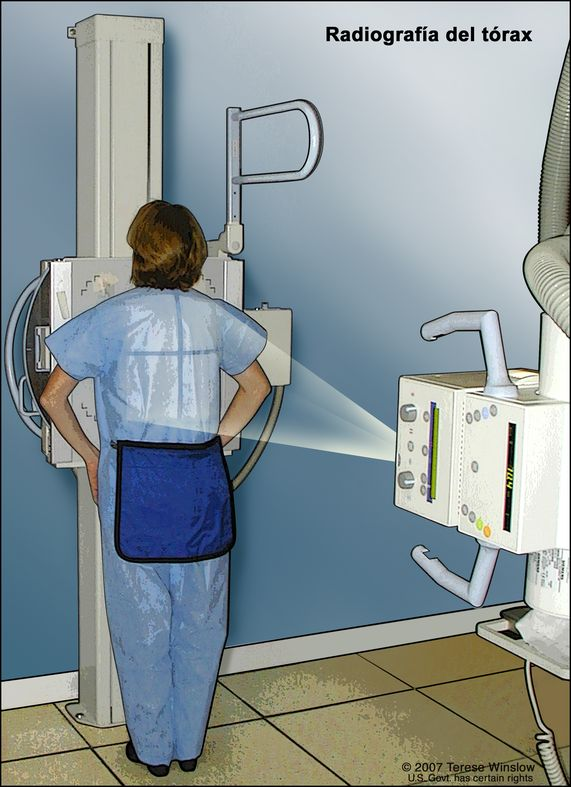
\includegraphics[width=0.44\textwidth]{img/radiografia torax.jpg}
    \caption{Ilustración CXT PA ~\cite{NIH24}}
    \label{fig:radiografia torax}
\end{figure}
\FloatBarrier

\subsection{Tomografía axial computarizada (TAC)}

El TAC es una técnica de diagnóstico por imágenes que emplea una máquina de rayos X conectada a una computadora para producir imágenes transversales del interior del cuerpo, con el fin de identificar una afección o planificar un tratamiento ~\cite{NIHTAC24}. 

El paciente se acuesta sobre una mesa (donde debe permanecer quieto) que se desplaza lentamente dentro de un escáner de rayos X en forma de anillo tal y como se aprecia en la imágen \ref{fig:TAC}. La computadora crea imágenes de la zona del cuerpo deseada en forma de cortes con las que se pueden crear modelos tridimensionales. En algunos casos, se requiere la introducción de contraste en el cuerpo por vía intravenosa o mediante la ingesta oral, para poder observar mejor algunas zonas ~\cite{MedPlusTAC24}.

Algunos riesgos de esta prueba incluyen la exposición a radiación o problemas derivados del contraste como alergias o daño a la función renal ~\cite{MedPlusTAC24}.

\begin{figure}[h]
    \centering
    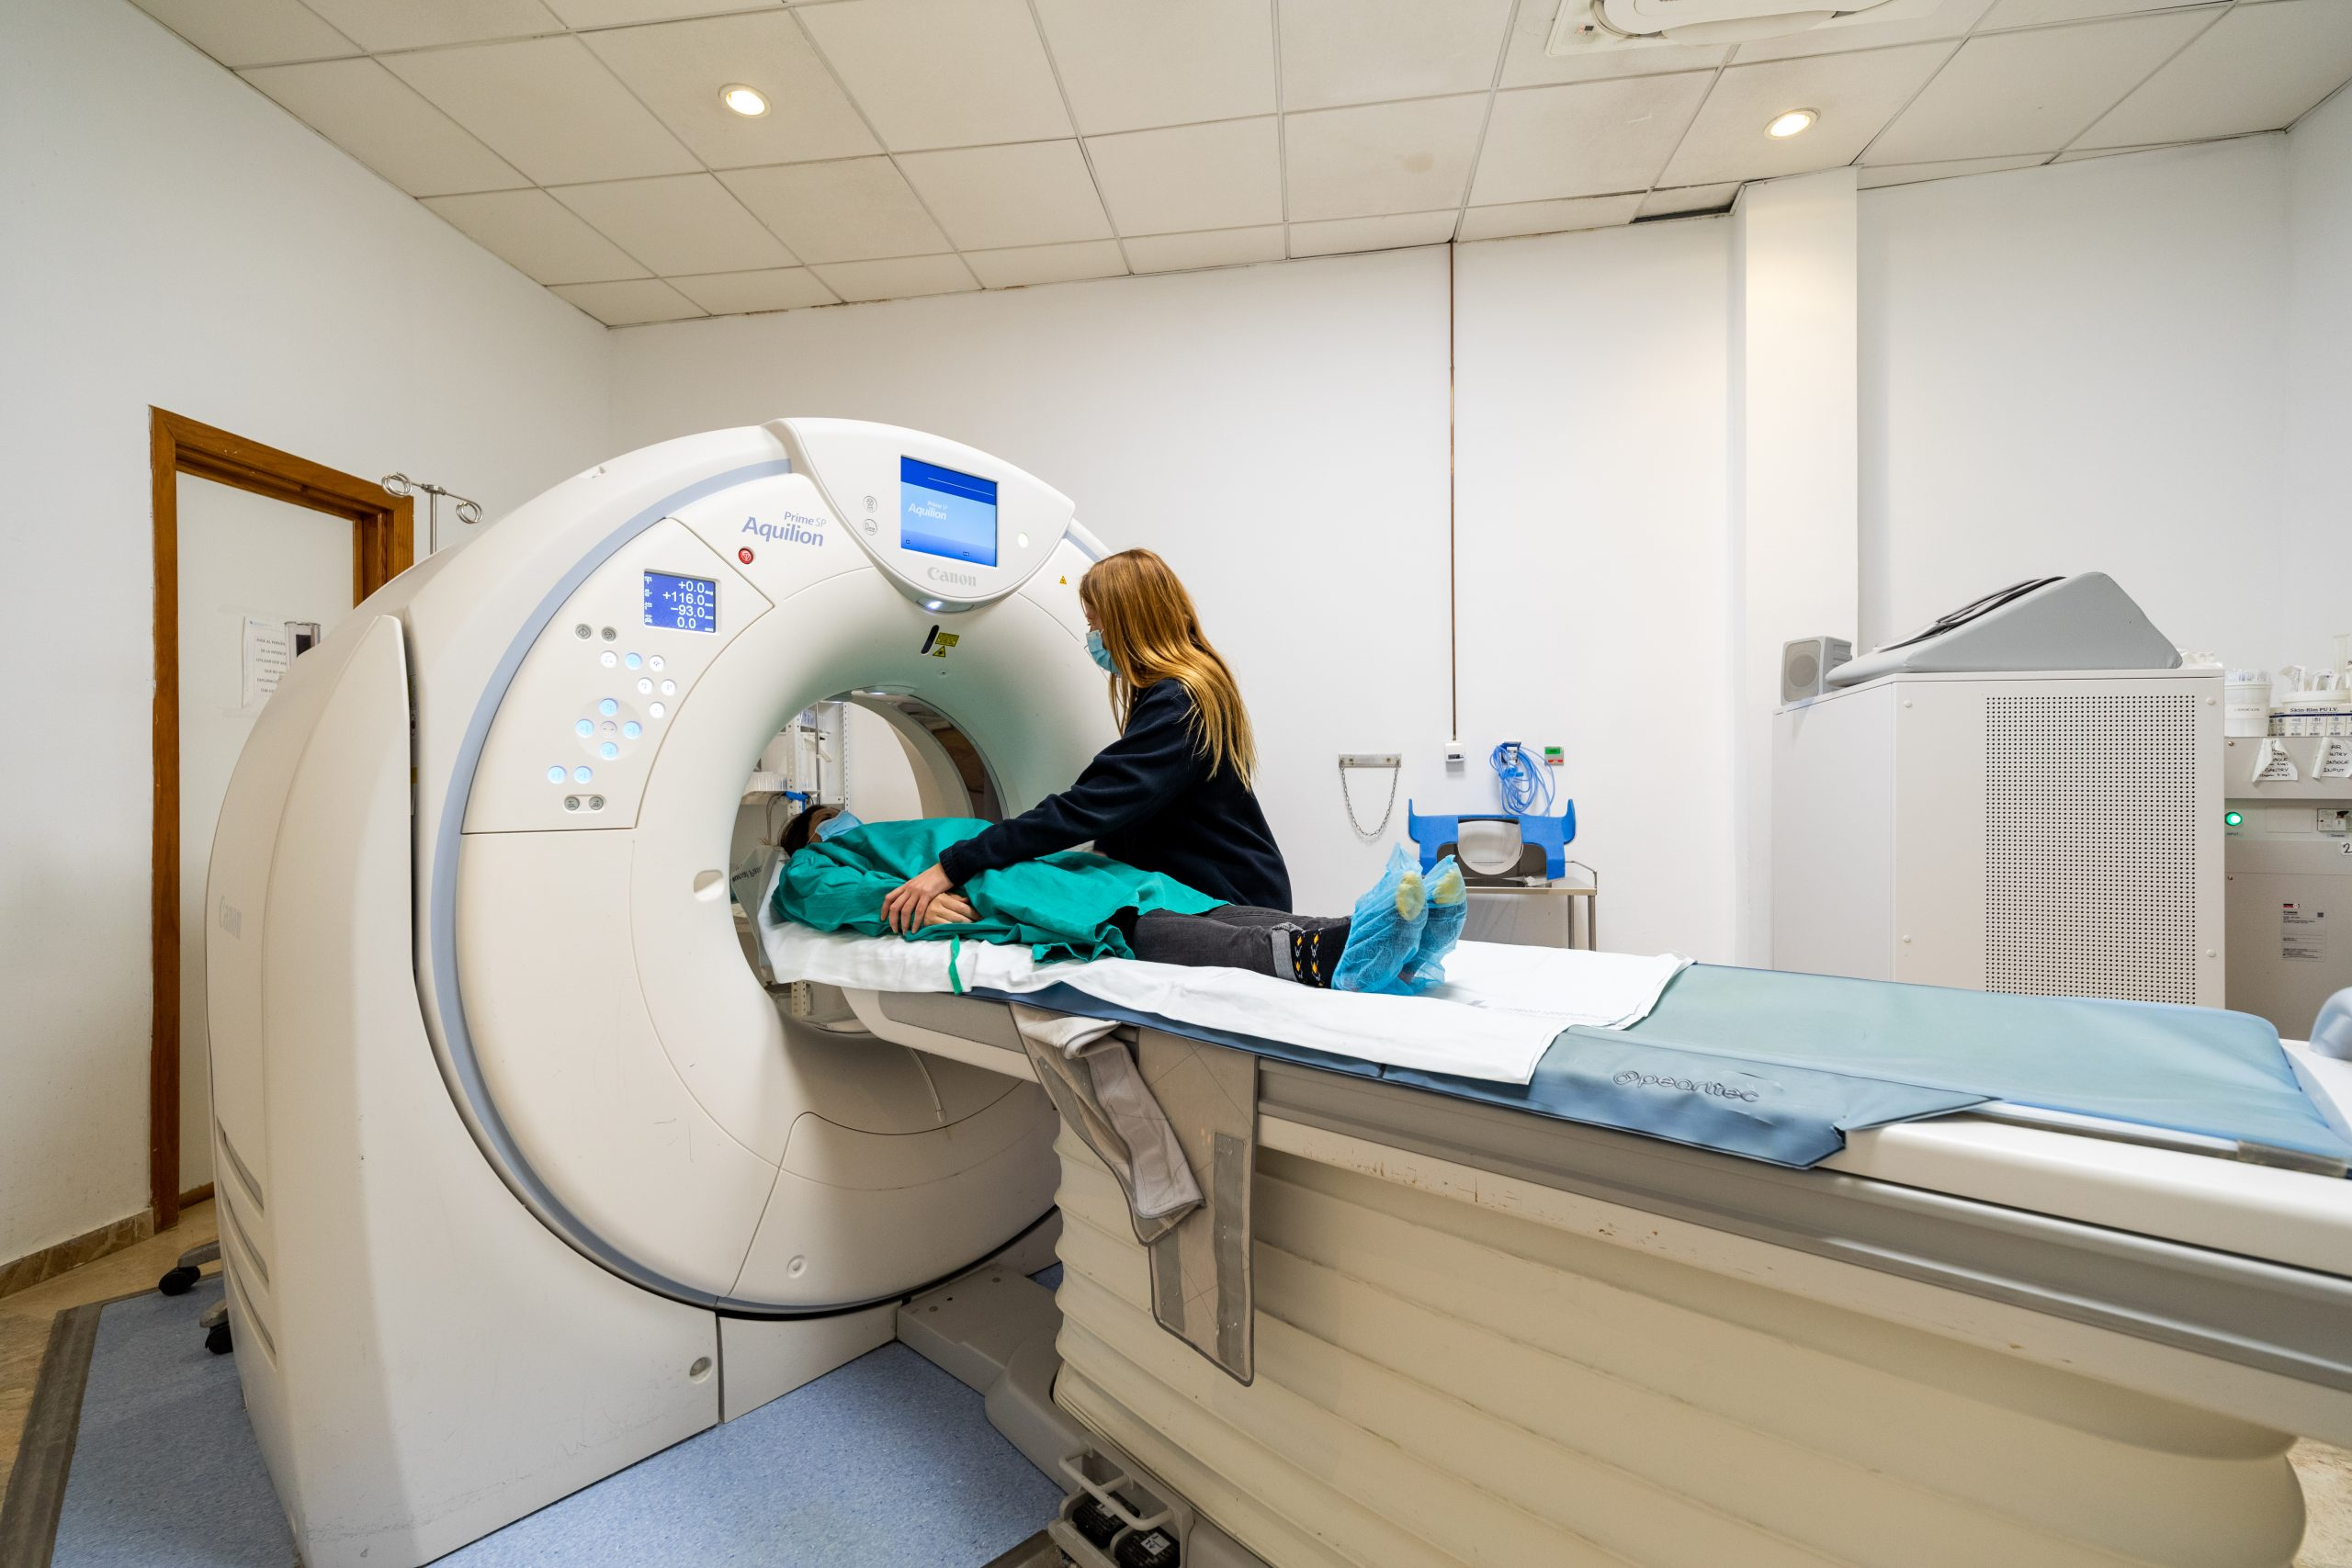
\includegraphics[width=0.70\textwidth]{img/TAC.jpg}
    \caption{Ilustración TAC ~\cite{HosPa24}}
    \label{fig:TAC}
\end{figure}
\FloatBarrier

\subsection{Opacidades blancas en la CXT}

La neumonía provoca inflamación de los alvéolos y derrame pleural, afección que consiste en una acumulación de líquido en los pulmones, lo que reduce la cantidad de oxígeno en el torrente sanguíneo provocando dificultades respiratorias ~\cite{kundu2021pneumonia}.

En una CXT, se puede diferenciar un estado saludable de un estado neumónico por anomalías como infiltrado pulmonar u opacidades blancas ya que, los pulmones sanos dejan pasar la radiación de los rayos X, por lo que se observan como zonas oscuras, a diferencia de los pulmones con algún tipo de anomalía ~\cite{gelaw15}.

Las opacidades blancas pueden ser causadas por multitud de patologías (entre ellas la neumonía) y presentan diversos patrones, algunos de ellos son:

\begin{itemize}
    \item \textbf{Consolidación}: opacidad homogénea de tamaño variable, con márgenes mal definidos e irregulares. Presenta broncograma aéreo, vías respiratorias llenas de aire vistas como líneas oscuras a través del pulmón opacificado ~\cite{gelaw15}.
    
    Su causa principal es la introducción de líquido o tejidos blandos en las vías respiratorios dificultando el paso del aire ~\cite{gelaw15}.
    
    La consolidación más típica es causada por neumonía bacteriana, aunque, también puede encontrarse en tuberculosis pulmonar\\ ~\cite{gelaw15}.
    
    \item \textbf{Colapso (atelectasias)}: opacidad y perdida de volumen que  puede afectar a los lóbulos, segmentos o subsegmentos del pulmón\\ ~\cite{gelaw15}.

    \item \textbf{Opacidades nodulares}: opacidades pequeñas y redondeadas causadas por diferentes patologías. Radiológicamente, su tamaño puede variar desde nódulos miliares (<2 mm) hasta masa pulmonar (>30 mm). Comúnmente son homogéneos (sin broncogramas aéreos) y sus bordes están bien definidos ~\cite{gelaw15, RadiopaediaPulmNodule24}.

    \item \textbf{Opacidades intersticiales}: opacidades que se observan como nódulos difusos,  sombras reticulares, reticulonodulares o líneas entrecruzadas, tal y como se puede apreciar en la figura \ref{fig:patrones_intersticial}  ~\cite{gelaw15}.

    \begin{figure}[h]
        \centering
        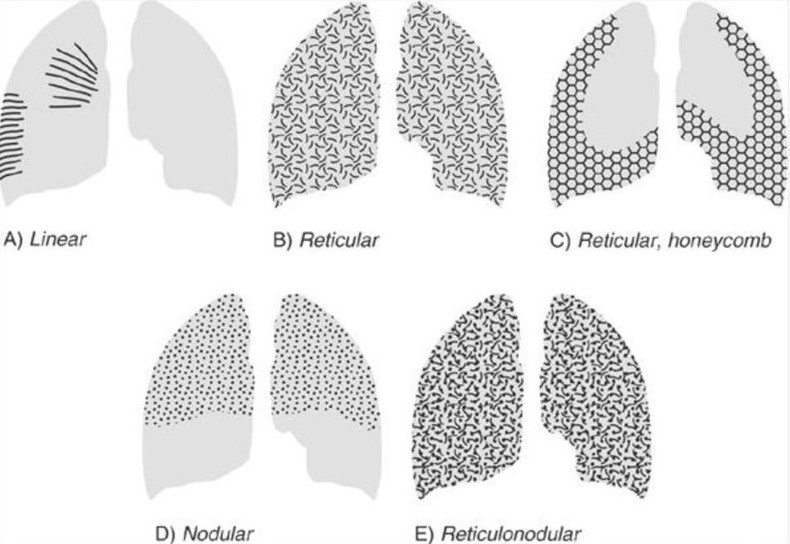
\includegraphics[width=0.99\textwidth]{img/patrones_intersticial.jpg}
        \caption{Clasificación patrón intersticial ~\cite{SlidePlayer24}}
        \label{fig:patrones_intersticial}
    \end{figure}
    \FloatBarrier
    
    Es el patrón más común de la enfermedad pulmonar intersticial difusa, la cual engloba un grupo de enfermedades pulmonares que afectan el intersticio (tejido conectivo que forma la estructura de soporte de los alvéolos) ~\cite{RadioInfo24}. Aunque, también puede verse en casos de tuberculosis en inmunocompetentes ~\cite{gelaw15}. 

    \item \textbf{Opacidades pleurales de la pared torácica}: pueden ser causadas por derrame pleural (líquido en la cavidad pleural), engrosamiento pleural (espesor de la pleura mayor de 3 mm), calcificación (proceso mediante el cual el calcio se acumula en el tejido corporal provocando que este endurezca) o por masa que surge del tejido blando ~\cite{gelaw15, MedlinePlusCalcificación24}. Se trata de un patrón típico de la tuberculosis.
    
\end{itemize}

Las características propias de la neumonía bacteriana para ser identificada  en una CXT son opacidades pulmonares focales segmentarias (es decir, bronconeumonía ) o lobares (es decir, neumonía lobar) \cite{RadiopaediaNeumoBact24}.

La bronconeumonía consiste en una inflamación peribronquiolar con posterior consolidación en el lóbulo pulmonar secundario. A nivel microscópico, la inflamación se puede ver como una congestión y dilatación extensa de los vasos sanguíneos y áreas de consolidación mal delimitadas \cite{RadiopaediaBronconeumonía24}.

La neumonía lobar está asociada con una consolidación homogénea y fibrosis o fisuras pulmonares de uno o más lóbulos de un pulmón. También presenta broncogramas aéreos \cite{RadiopaediaPulmLobar24}.

\section{Estado del arte y trabajos relacionados.}

\subsection{Prevalencia de la neumonía}

La neumonía es una infección respiratoria aguda que afecta a las vías respiratorias y a los alvéolos ~\cite{antoni2021}. 

A diferencia de otras patologías, la neumonía, no depende del grupo de edad ni de la parte del mundo ya que, presenta altas tasas de mortalidad y morbilidad en todos los grupos de edad y en todas las partes del mundo. Aunque, por un lado, tiene una mayor prevalencia en niños menores de cinco años y adultos mayores de sesenta y cinco años con enfermedades previas y, por otro lado, la prevalencia también varía según el lugar geográfico ~\cite{antoni2021}. 

En 2019, la neumonía causó más de 2,5 millones de muertes en todo el mundo, lo que la convirtió en la principal causa de mortalidad por enfermedades infecciosas por encima de la tuberculosis y el VIH ~\cite{shi2020global}. Teniendo África unas tasas de mortalidad mayores respecto a Europa y Estados Unidos (EE. UU) ~\cite{lim2022pneumonia}. Esto puede deberse a que en los países en desarrollo o subdesarrollados existe un alto nivel de contaminación, infraestructuras médicas inadecuadas y escasez de medidas higiénicas ~\cite{kundu2021pneumonia}

En EE. UU, un estudio publicado en 2015 determinó que la incidencia de neumonía adquirida en la comunidad (NAC) fue de 6,3 por cada 1000 habitantes en adultos de entre 65 y 79 años y de 16,4 por cada 1000 habitantes en adultos de más de 80 años ~\cite{jain2015community}.

En Europa, un estudio publicado en 2013 determinó que la incidencia fue de 14 por cada 1000 habitantes siendo predominante en hombres ~\cite{torres2013risk}. 

Estas diferencias entre zonas pueden deberse a los distintos sistemas sanitarios, la disminución del tabaquismo en EE. UU entre 2005 y 2016 o una vacuna neumocócica recibida en EE. UU, entre otros posibles factores. Sin embargo, la epidemiología de la neumonía manifiesta un cambio constante debido a nuevas terapias, diversas de pruebas, etc. Aunque, desde principios del siglo XXI, ha sido la causa más común de infecciones pandémicas ~\cite{jain2015community}. 

La predominancia de padecer NAC en hombres respecto a mujeres puede deberse a factores conductuales, socioeconómicos o diferencias en la anatomía ~\cite{antoni2021}. 

Además, la neumonía es la principal causa de muerte en niños menores de 5 años, con una mortalidad de 2.400 niños por día. Esta alta mortalidad puede deberse a una mayor debilidad en sus sistemas inmunológicos debido a un menor desarrollo ~\cite{saboo23}.

Las tasas de ingreso en las unidades de cuidados intensivos (UCI) difieren en distintas partes del mundo según los recursos disponibles y sus políticas de admisión. Por ejemplo, en América del Norte, más del 15\% de los pacientes hospitalizados son trasladados a la UCI, mientras que, en Europa esta cifra oscila entre el 5\% y el 10\% ~\cite{lim2022pneumonia}.

Por ello, este trabajo puede ser de gran ayuda para erradicar las distinciones entre lugares del mundo con distintas posibilidades, consiguiendo un mejor diagnóstico médico independientemente de la situación económica, social, etc. de ese país.

\subsection{Causas y tipos}

Entre las principales causas de la neumonía se encuentran las bacterias, virus respiratorios y hongos. La neumonía bacteriana, es generalmente causada por microorganismos que van desde la nasofaringe hasta el tracto respiratorio inferior ~\cite{antoni2021}.

Los patógenos se pueden transmitir entre individuos. Se trata de una infección altamente contagiosa. Además, las probabilidades de infección aumentan, en función de la existencia de algunos factores tales como, las defensas del huésped alteradas (o deficientes), la existencia de otra infección, enfermedades pulmonares previas, o un microorganismo altamente virulento ~\cite{antoni2021}.

Existen dos tipos principales de neumonía, la neumonía adquirida en la comunidad (NAC) y la adquirida en el hospital (NAH), esta última incluye la neumonía asociada a la ventilación (NAV). La NAC, a diferencia de la NAH, se contrae fuera del entorno hospitalario, en lugares como el hogar, el trabajo, el colegio, etc ~\cite{antoni2021}.

Dado que, la forma de adquirir la neumonía es distinta en NAC y NAH, las causas también son diferentes ya que, NAC es causada principalmente por \textit{Streptococcus pneumoniae}, virus respiratorios, \textit{Haemophilus influenzae} y otras bacterias como \textit{Mycoplasma pneumoniae} y \textit{Legionella pneumophila} mientras que, en el caso de NAH, las principales causan son \textit{Staphylococcus aureus}, \textit{enterobacterales}, \textit{bacilos gramnegativos no fermentadores}, y \textit{Acinetobacter spp} ~\cite{antoni2021}.

En algunos casos, la NAC puede ser causada por bacterias MRSA (resistentes a antibióticos). En estos casos el tratamiento se complica para los médicos ya que, deben identificar los factores de riesgo para estos patógenos y realizar una terapia personalizada adecuada ~\cite{antoni2021}. La NAH también puede ser causada por patógenos resistentes a medicamentos, cuya infección es más probable a medida que aumentan los días del paciente en el hospital ~\cite{lim2022pneumonia}.

Entre las características de la \textbf{neumonía bacteriana} se pueden destacar las siguientes:
\begin{itemize}
    \item Opacificación densa y bien definida en un lóbulo pulmonar.
    \item Puede existir broncograma aérea, lo que significa que, los bronquios llenos de aire son visibles dentro de una consolidación.
    \item Puede haber acumulación de líquido en el espacio pleural (derrame pleural).
\end{itemize}

Por el contrario, entre las características de la \textbf{neumonía viral}, se encuentran las siguientes:
\begin{itemize}
    \item Presentan un patrón más difuso y reticular, afectando más el intersticio pulmonar.
    \item Se pueden observar colapsos parciales del pulmón (atelectasias).
    \item Los infiltrados suelen ser bilaterales ya que, afectan a ambos pulmones de una forma más difusa.
\end{itemize}


\subsection{Síntomas y complicaciones}

Los síntomas de la neumonía incluyen dificultad para respirar, tos, disnea, dolor en el pecho, fatiga, fiebre y producción de esputo ~\cite{lim2022pneumonia}. 

A su vez, la neumonía puede estar ligada a otras complicaciones. Entre el 36\% y el 48\% de los pacientes hospitalizados por neumonía desarrollan sepsis, una disfunción orgánica potencialmente mortal causada por una respuesta desregulada del huésped a una infección ~\cite{ManualMSD24}. 

El sistema cardiovascular también se ve afectado dado que, un gran número de pacientes hospitalizados por neumonía sufre de problemas cardiovasculares tales como insuficiencias cardiacas, arritmias o síndrome coronarios agudos dentro de los siete días siguientes al diagnóstico de la neumonía ~\cite{antoni2021}. Algunos estudios también han demostrado que la neumonía aumenta en un 57\% el riesgo de padecer demencia ~\cite{shah2013bidirectional}. Cabe destacar que, la neumonía puede ser algo recurrente ya que, la tasa de reingreso de pacientes con NAC varía entre un 16,8\% y un 20,1\% ~\cite{antoni2021}.


\subsection{Factores de riesgo y prevención}

Los factores de riesgo de NAC varían en niños y adultos. En el caso de los niños, los principales factores de riesgo son la prematuridad, la desnutrición, una lactancia materna subóptima y la contaminación en las casas ~\cite{antoni2021}.
En el caso de los adultos, algunas enfermedades como la diabetes mellitus, enfermedades hepáticas y enfermedades cardiovasculares se manifiestan como los principales factores de riesgo de NAC. Otro factor de riesgo importante es la inmunocompetencia, ya que, pacientes cuyas defensas inmunitarias contra las infecciones están debilitadas presentan un mayor riesgo de NAC. Un estilo de vida poco saludable es otro factor de riesgo ya que, el tabaquismo, el alcohol o una dieta poco sana están asociados con la NAC ~\cite{antoni2021}. 

Por lo tanto, algunas maneras de prevenir la NAC implican no fumar ni beber alcohol, realizar ejercicio físico, una correcta higiene dental, evitar el contacto con niños con infecciones respiratorias y vacunarse contra la influenza y el neumococo ~\cite{lim2022pneumonia}.

En cuanto a los factores de riesgo y la mayoría de las prevenciones de la NAH, están asociadas a otros riesgos y, aún no han sido probadas. Un ejemplo de esto es, el uso de antibióticos para la descontaminación oral o digestiva que, puede ser eficaz, pero, también puede aumentar la resistencia a antibióticos. Otro ejemplo consiste en el empleo de clorhexidina para el lavado bucal, el cual puede ayudar a prevenir la NAH, aunque, estudios recientes han demostrado una mayor mortalidad en pacientes que recibieron clorhexidina ~\cite{antoni2021}.

\subsection{Tratamiento}

El lugar de recuperación de un paciente con NAC depende de su gravedad en función de una serie de factores como su frecuencia respiratoria, nivel de nitrógeno ureico en sangre, presión arterial y edad. De menor a mayor gravedad se consideran las siguientes pautas: tratamiento ambulatorio, estancia hospitalaria corta u observación cercana y hospitalización, llegando a una posible atención en la UCI en los casos más graves ~\cite{file2023community}. 

En pacientes inmunocomprometidos, los signos y síntomas usuales de una enfermedad grave pueden estar ausentes. Por ello, se requiere una vigilancia más cuidadosa y constante ~\cite{lim2022pneumonia}.

Para un correcto tratamiento de la neumonía, lo ideal es emplear biomarcadores para distinguir entre una neumonía viral o no infecciosa y una neumonía bacteriana a partir de la respuesta inmunológica del huésped. Ya que, en el caso de la primera opción no se requiere de antibiótico mientras que en la segunda sí. Pero, esto se complica en el caso de pacientes con el sistema inmunológico alterado ~\cite{lim2022pneumonia}. 

La procalcitonina es un precursor de la calcitonina (hormona peptídica involucrada en la homeostasis del calcio) sintetizado fundamentalmente en las células C del tiroides, pero también, en menor medida, en órganos como pulmones e intestino. En condiciones normales, sus niveles son bajos, pero aumentan significativamente en respuesta a infecciones bacterianas sistémicas y sepsis. La prueba de la procalcitonina se emplea para determinar si se trata de una NAC bacteriana o viral ya que, la procalcitonina es desencadenada por citocinas específicas en respuesta a bacterias. Sin embargo, a la hora de realizar la prueba de la procalcitonina también se pueden dar falsos positivos por lo que, no se deben interpretar los niveles de procalcitonina como indicadores definitivos ~\cite{file2023community}.

En el caso de la neumonía bacteriana, es preferible que el tratamiento esté dirigido específicamente al patógeno causante de la neumonía, sin embargo, normalmente, no se puede identificar este patógeno con rapidez. Por lo que, para comenzar con la terapia lo antes posible, se realiza una terapia empírica (es decir, sin conocimiento preciso de la causa o la naturaleza de la afección) que cubra los patógenos etiológicos más probables. Una vez que se obtienen los resultados de las pruebas diagnósticas (que tardan entre 48 y 72 horas), se ajusta el tratamiento para que sea específico para el patógeno identificado. Gracias a los avances en ciencia y tecnología existen nuevos métodos aprobados por la FDA (Administración de Alimentos y Medicamentos de los Estados Unidos) que proporcionan los resultados de las pruebas de diagnóstico en un plazo de 2 a 4,5 horas o incluso menos, de esta manera, se facilita un tratamiento más preciso evitando el uso innecesario o inapropiado de antibióticos ~\cite{antoni2021}.

A la hora de elegir la terapia empírica, es muy importante tener en cuenta algunos factores del paciente tales como datos epidemiológicos, enfermedades en los pulmones, corazón o hígado, diabetes, trastorno por consumo de alcohol, hospitalización reciente, lugar de adquisición de la neumonía, etc. También, hay que tener en cuenta la dosis y la vía de administración adecuadas dependiendo de la infección ~\cite{antoni2021}.  En presencia de factores de riesgo, se recomienda iniciar la terapia empírica dirigida a MRSA ~\cite{file2023community}.

En el caso de NAC grave, algunos pacientes pueden recibir corticosteroides como terapia complementaria. Esta terapia está aún en evolución, pero con evidencias positivas recientes de beneficios en pacientes con NAC grave. Se debe evitar esta terapia en pacientes con una posible gripe, influenza o neumonía por Aspergillus ~\cite{file2023community}.

Alrededor de un tercio de los pacientes con neumonía, presentan una infección con más de un patógeno. Generalmente se trata de combinaciones de patógenos bacterianos y virales ~\cite{lim2022pneumonia}.

Cabe mencionar que, aunque con un correcto tratamiento, los síntomas de la neumonía comienzan a mejorar rápidamente (dependiendo de la gravedad), no es, hasta después de 6 meses, que se logra la recuperación completa en algunos casos de NAC leve. Sin embargo, en otros casos, no se llega a conseguir una recuperación del 100\% ya que, se han observado en múltiples pacientes complicaciones cardíacas y respiratorias derivadas de la neumonía, lo que desemboca en una peor calidad de vida y un mayor grado de mortalidad a largo plazo ~\cite{antoni2021}. 

En el caso de hospitalización, el alta hospitalaria se produce cuando el paciente se encuentra clínicamente estable, puede continuar el cuidado en un entorno seguro y puede tomar medicamentos por vía oral. Se promueve el alta temprana para evitar riesgos asociados con la hospitalización, además de la reducción de costes. Pero, el paciente mantiene un seguimiento para evitar un posible reingreso en el hospital ~\cite{file2023community}.

La duración del tratamiento depende de cada caso, aunque, por lo general, suele estar entorno a un mínimo de 5 días. Este tiempo se prolonga en caso de complicaciones, pacientes con condiciones inmunocomprometidas, etc ~\cite{file2023community}.

\subsection{Diagnóstico}

El diagnóstico precoz es fundamental para poder obtener buenos resultados en el tratamiento por lo que, pruebas de diagnóstico rápidas y precisas mejoran el tratamiento ~\cite{antoni2021}. Un ejemplo de esto es que, en pacientes gravemente enfermos, iniciar el tratamiento lo antes posible, está relacionado con un menor porcentaje de mortalidad ~\cite{lim2022pneumonia}.

La CXT es el método más empleado en todo el mundo para el diagnóstico de la neumonía debido a su bajo costo y la facilidad de acceso ~\cite{li2020accuracy}. Es esencial para un correcto diagnóstico ya que, aporta información acerca del lugar concreto donde se encuentra la neumonía en el pulmón, su extensión o las características asociadas. Es de gran ayuda en la detección de opacidades pulmonares, los cuales sirven como indicadores de gravedad. Aunque, en ocasiones, es necesario complementar la CXT con la TC para una mejor detección ya que, hay infiltrados pulmonares que una CXT simple no es capaz de detectar, por ejemplo, cuando existe una neumonía recurrente, carcinoma del pulmón o empiema (pus en la capa que recubre los pulmones) ~\cite{antoni2021}.

A pesar de que la CXT sea el método más empleado en la detección de la neumonía, existen discordancias por parte de algunas personas sobre su uso ~\cite{wootton2014diagnosis}.

En el contexto comunitario, en determinadas áreas, existen desacuerdos ente realizar una CXT para confirmar un diagnóstico con sospecha de neumonía o aplicar un tratamiento empírico y, solo en caso de que este no mejore, realizar la radiografía. Esto lo hacen debido a su coste, las posibles molestias causadas al paciente, posibilidad de retraso en el diagnóstico y falta de disponibilidad inmediata para realizar una radiografía de rutina ~\cite{wootton2014diagnosis}. 

Previamente se ha comentado que, la CXT tiene un bajo coste y es no invasiva. Pero, en este caso, con el coste radiológico se refiere a la infraestructura necesaria para realizar la radiografía (que incluye equipo de rayos X y personal sanitario necesario para realizar y analizar la radiografía) ya que, ese coste puedo ser muy relevante en algunos lugares donde el acceso a la atención médica es limitado. Y, respecto a las molestias para el paciente, si bien es cierto que la CXT debería ser lo más segura posible evitando exponer al paciente todo lo que se pueda a la radiación y no es una prueba especialmente molesta, sí que existe una breve exposición a la radiación ionizante, lo que puede ser percibido como una molestia o preocupación por parte de algunas personas, especialmente si tienen que realizarse múltiples radiografías en un corto período de tiempo. Además, pueden existir molestias físicas asociadas con la posición requerida para la obtención de la imagen ~\cite{wootton2014diagnosis}.  Las diferentes posturas necesarias a la hora de realizar una CXT están correctamente explicadas en el \textit{Anexo D}.  

Hay que añadir que, al margen de las dificultades comentadas previamente por las que, en algunos lugares, en vez de realizar CXT, se basan exclusivamente en los síntomas para establecer un tratamiento, hay quien piensa que, la realización de una CXT es completamente innecesaria en algunos casos. Esta opinión se basa en las limitaciones diagnósticas de la CXT y la dificultad para interpretar dichas imágenes, especialmente por la presencia de puntos ciegos, anomalías demasiado sutiles o similitudes radiológicas con otras afecciones. Por lo que, prefieren fiarse del juicio clínico (basado en los síntomas del paciente) ~\cite{wootton2014diagnosis}.

Sin embargo, en el entorno hospitalario la CXT se realiza de manera rutinaria para confirmar el diagnóstico, y, está asociado con un beneficio clínico, lo que demuestra su importancia. También se mantiene el pensamiento de que, a pesar de los inconvenientes mencionados previamente, una CXT debería ser un requisito imprescindible para diagnosticar correctamente la neumonía (aunque, en ciertos lugares esto no puede hacerse debido a sus bajos recursos). Debido a que, se ha demostrado que un gran porcentaje de pacientes que no eran diagnosticados con neumonía basándose únicamente en sus síntomas, fueron diagnosticados con neumonías tras la realización de una CXT y, lo mismo ocurría en el caso contrario (personas sin neumonía diagnosticadas con neumonía por sus síntomas) ~\cite{wootton2014diagnosis}. Por lo que, esto no es más que un ejemplo donde se refleja la necesidad de implementar una red neuronal para la identificación de neumonía a partir de CXT que pueda ser llevada al ámbito clínico para acabar con los problemas de coste, personal y mal diagnóstico en zonas menos desarrolladas.

Otro ejemplo de esto es que, en un estudio realizado en la periferia norte de Israel, donde no existe una gran accesibilidad a las instalaciones de radiología, se ha demostrado que, la confirmación de un diagnóstico clínico de neumonía empleando CXT es fundamental ya que, en muchos casos, por falta de  accesibilidad a dichas instalaciones se diagnostica como neumonía y se trata con antibióticos a pacientes que, posteriormente con una CXT se ha demostrado que no tenían neumonía, lo que conlleva una prescripción excesiva de antibióticos y un posible desarrollo futuro de resistencia a los antibióticos ~\cite{eilat2022community}.

La ecografía pulmonar es otro método diagnóstico para la obtención de imágenes de forma no invasiva ya que, no se produce exposición a la radiación (a diferencia de la TC) y tiene un fácil empleo, aunque, puede presentar limitaciones a la hora de estudiar las capas más profundas, lo que dificulta el diagnóstico de algunas afecciones ~\cite{antoni2021}.

En el caso de pacientes hospitalizados por neumonía, es recomendable la realización de una serie de pruebas de laboratorio para un correcto diagnóstico e identificación de patógenos. Entre estas pruebas se encuentran muestras de esputo (o flema) para detectar bacterias o gérmenes que puedan causar una infección pulmonar, muestras de sangre, muestras respiratorias distales como BAL (lavado bronquio alveolar) o PCR viral en hisopos faríngeos. Esta última, se realizó sobre todo en la pandemia COVID-19 para la detección de SARS-COV-2 ~\cite{antoni2021}. En atención primaria, es poco común la realización este tipo de pruebas debido a la limitada disponibilidad de laboratorios y los tiempos prolongados para la obtención de resultados ~\cite{lim2022pneumonia}.

Algo muy importante a tener en cuenta es que, no siempre se realiza un correcto diagnóstico de la neumonía debido a su similitud tanto a nivel de características radiográficas como a nivel de sintomatología con otras afecciones pulmonares ~\cite{lim2022pneumonia}.

\subsection{Implicación del \textit{deep learning} en el diagnóstico de neumonía}

Como ya se ha comentado previamente, las radiografías de tórax proporcionan una gran cantidad de información para el diagnóstico de la neumonía, aunque, en muchas ocasiones, identificarla se vuelve muy difícil incluso para radiólogos experimentados debido a las semejanzas radiográficas que esta afección puede tener con otras afecciones como cáncer de pulmón o acumulación de líquido ~\cite{li2020accuracy}. Otros factores como la profundidad de la inspiración o la posición del paciente también dificultan la interpretación de dichas imágenes ~\cite{jaiswal2019identifying}. Por ello, el diagnóstico de la neumonía a partir de una CXT por el método tradicional, es decir, mediante la identificación de la neumonía por parte del médico a partir de la imagen, no es preciso e implica tiempo. Esto, puede derivar en un mal diagnóstico o en el retraso del tratamiento, lo que implica un empeoramiento del estado del paciente y un aumento de las tasas de morbilidad y mortalidad ~\cite{li2020accuracy}.

Por eso, a partir de los avances científicos y tecnológicos de los últimos años se ha propuesto ayudar a los médicos en la interpretación de esas imágenes con sistemas de detección asistida por computadora (CAD) basados en IA ~\cite{li2020accuracy}.

El aprendizaje profundo o DL (por sus siglas en inglés), tiene un alto potencial en el análisis de imágenes médicas gracias a su capacidad para reemplazar el proceso manual de identificación y clasificación de características en imágenes de radiografías de tórax. Su éxito, se debe principalmente a la capacidad de las redes neuronales para aprender conceptos complejos a partir de datos nuevos en un proceso de aprendizaje. Además de la detección de neumonía a partir de la CXT, el DL ha realizado avances también en el análisis de imágenes para otras afecciones como retinopatía diabética, arritmias y cáncer ~\cite{li2020accuracy}.

Se han llevado a cabo diversos algoritmos por parte de los investigadores para el análisis de las imágenes de rayos X ~\cite{jaiswal2019identifying}. Sin embargo, aún se tienen que realizar numerosos avances antes de poder incorporar el DL en el entorno clínico. Esto incluye, la precisión de los algoritmos, el correcto ajuste de los hiperparámetros, como el tamaño del lote, el número de épocas, la tasa de aprendizaje y el número de capas en las redes neuronales. Además, la cantidad y calidad del conjunto de datos juega un papel crucial. Otros aspectos importantes incluyen, el tiempo de cálculo y la tasa de error. Solo cuando se mejoren estos aspectos en su totalidad, se podrá considerar la viabilidad de llevar estos algoritmos al ámbito clínico ~\cite{jaiswal2019identifying, sharma2024systematic}.

Uno de los grandes problemas a los que se han enfrentado los investigadores es la cantidad de datos limitada ya que, al trabajar con modelos previamente entrenados, se necesitan grandes cantidades de datos además de hiperparámetros configurados correctamente para obtener los mejores resultados. Trabajar con un gran número de imágenes etiquetadas es fundamental para una correcta clasificación y predicción. Se han aplicado algunos métodos para el aumento de datos como voltear, rotar, recortar, escalar, trasladar y deformar elásticamente las imágenes para así, obtener un mayor número de imágenes ~\cite{sharma2024systematic}.

Para concluir, se puede afirmar que, existe una gran necesidad de investigación y un gran potencial de mejora en el ámbito de detección de neumonía a partir de técnicas de aprendizaje profundo ~\cite{sharma2024systematic}.



